The idea here is to describe the synaptic interaction in a more
realistic way: this can be achieved via biophysical models
partially describing the biochemical reactions involved. In particular,
two events are to be taken into account:
\begin{itemize}
    \item \textbf{Presynaptic Stage}: model the release of
          neurotransmitters kinetics.
    \item \textbf{Postsynaptic Stage}: model the synaptic current
          and synaptic receptors.
\end{itemize}
Roughly speaking, a biophysical model should take into account:
\begin{enumerate}
    \item The neurotransmitters release.
    \item The neurotransmitters diffusion.
    \item The neurotransmitters-receptors binding.
    \item The opening of channels.
\end{enumerate}
When talking about synapses kinetics schemes, there are four
different mechanisms, listed in the table below.
\begin{figure}[H]
    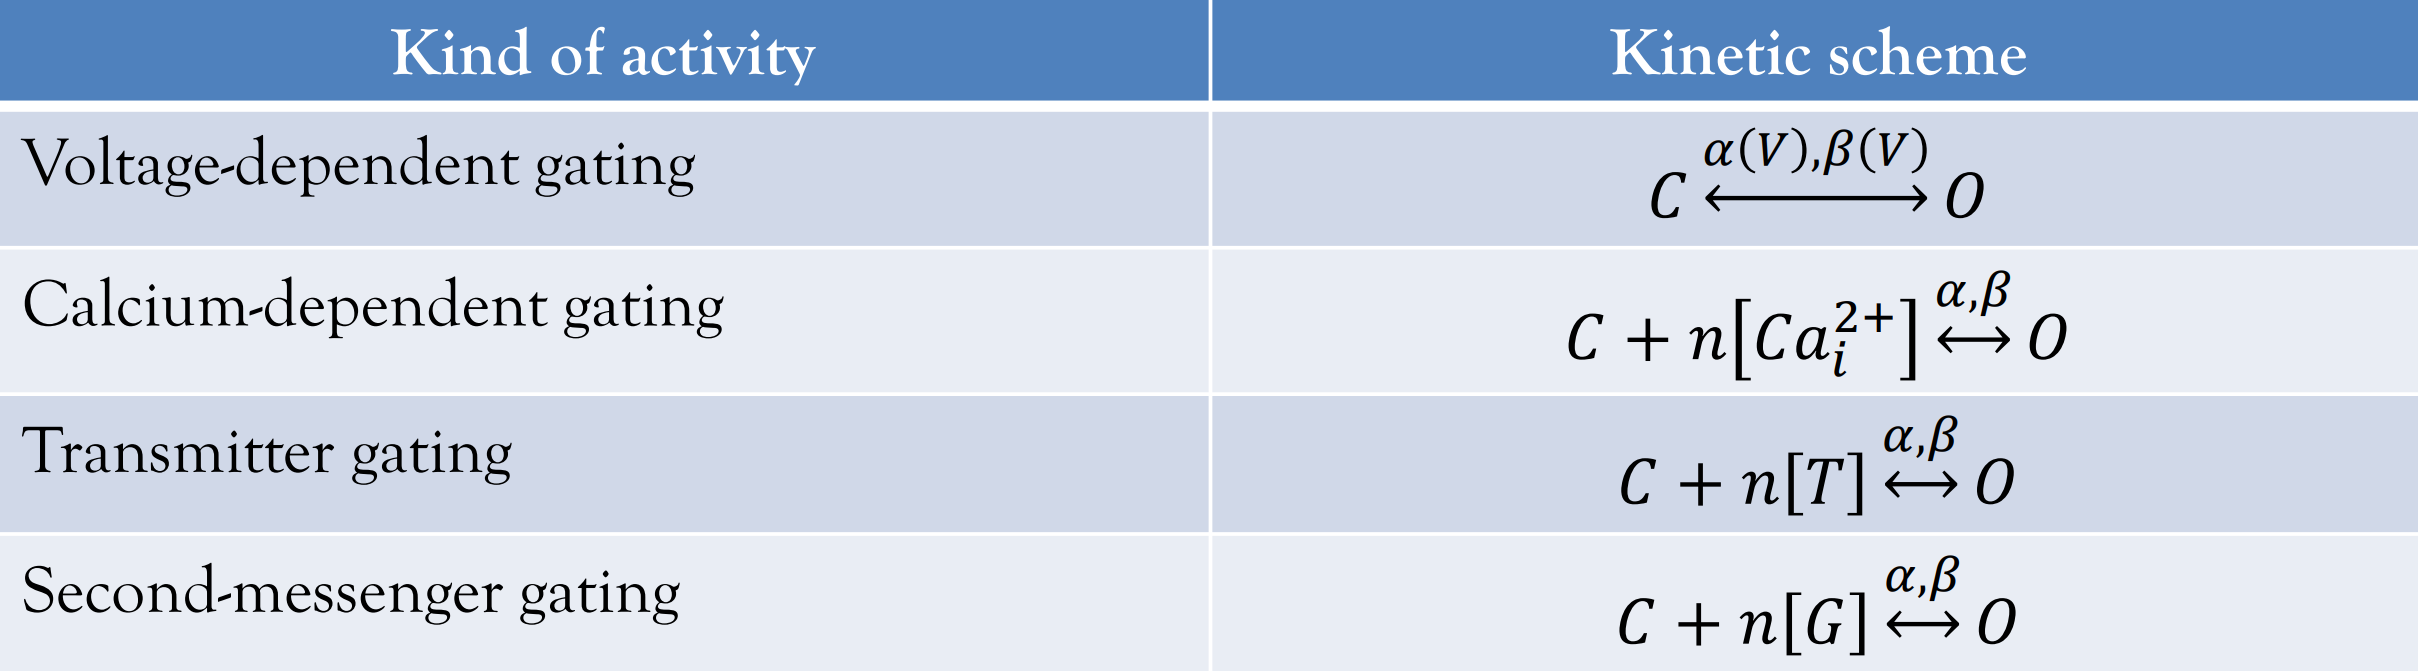
\includegraphics[scale=0.25]{13_1}
    \centering
\end{figure}
Note that \(C\) and \(O\) represent the closed and open conditions
respectively, while \([T]\) is the concentration of neurotransmitters and
\([G]\) the concentration on second-messengers.

\subsection{The Destexhe Model}
This is a model which aims at modelling ionotropic fast synapses, moreover
it is especially simple from the Computational point of view. The idea is to
better model the synaptic conductance \(g_{syn}(t)\) when the
neurotransmitters bind to the postsynaptic receptors, thus it
acts at the postsynaptic level, without taking into account the
behaviour of the presynaptic neuron.\\
First of all, let's write the expression of the synaptic conductance:
\begin{equation*}
    g_{syn}(t)=\bar{g}_{syn}\cdot{r(t)}
\end{equation*}
with \(r(t)\) is the fraction of bounded receptors, evolving over time.
From this, the synaptic current can be derived as usual:
\begin{equation*}
    I_{syn}=g_{syn}(t)\cdot{(V_{m}-E_{syn})}=\bar{g}_{syn}\cdot{r(t)}\cdot{(V_{m}-E_{syn})}
\end{equation*}
\paragraph{How is \(r(t)\) computed?} Let's in the first place write the
following relationship:
\begin{equation*}
    [R]+[T]\xleftrightarrow{\alpha,\,\beta}[TR^{*}]
\end{equation*}
where \([R]\), \([T]\) and \([TR^{*}]\) are the concentrations of
not-binding receptors, neurotransmitters, and binding-receptors respectively
and \(\alpha\) and \(\beta\) are parameters defining how the binding of receptors
and neurotransmitters occurs.
Then, if \([R_{0}]=[R]+[TR^{*}]\) is the total concentration of available receptors, the
fraction of bounded receptors \(r(t)\) can be defined as:
\begin{equation*}
    r(t)=\frac{[TR^{*}]}{[R_{0}]}
    \Rightarrow
    [TR^{*}]=[R_{0}]\cdot{r(t)}
\end{equation*}
Said so, the variation of \([TR^{*}]\) over time can be expressed as:
\begin{equation*}
    \frac{d[TR^{*}]}{dt}=\alpha{[R][T]}-\beta{[TR^{*}]}
\end{equation*}
By substituting \([TR^{*}]\), one would obtain:
\begin{equation*}
    \frac{d[TR^{*}]}{dt}=[R_{0}]\frac{dr(t)}{dt}
    \Rightarrow
    \frac{dr(t)}{dt}=\frac{1}{[R_{0}]}\frac{d[TR^{*}]}{dt}
\end{equation*}
Let's now carry on the following passages and substitutions:
\begin{align*}
    \frac{dr(t)}{dt}
    =\frac{1}{[R_{0}]}\frac{d[TR^{*}]}{dt}
     & =\frac{1}{[R_{0}]}\Bigl\{\alpha[R][T]-\beta[TR^{*}]\Bigr\}                              \\
     & =\alpha[T]\frac{[R]}{[R_{0}]}-\beta\frac{[TR^{*}]}{[R_{0}]}                             \\
     & =\alpha[T]\frac{[R]}{[R_{0}]}-\beta\frac{\cancel{[R_{0}]}\cdot{r(t)}}{\cancel{[R_{0}]}}
    =\alpha[T]\frac{[R]}{[R_{0}]}-\beta\cdot{r(t)}
\end{align*}
By recalling that \([R_{0}]=[R]+[TR^{*}]\) and that \([TR^{*}]=[R_{0}]\cdot{r(t)}\), the
following relationship holds:
\begin{equation*}
    [R_{0}]=[R]+[R_{0}]\cdot{r(t)}
    \Rightarrow
    [R]=[R_{0}]\bigl[1-r(t)\bigr]
    \Rightarrow
    \frac{[R]}{[R_{0}]}=1-r(t)
\end{equation*}
Finally, the following equation can be derived:
\begin{equation*}
    \frac{dr(t)}{dt}=\alpha[T]\cdot\bigl[1-r(t)\bigr]-\beta\cdot{r(t)}
\end{equation*}
Now, it is possible to write the following differential equation with a boundary
condition which describes the temporal evolution of bounded receptors at the postsynaptic level:
\begin{equation*}
    \begin{cases}
        \frac{dr(t)}{dt}=\alpha[T]\cdot\bigl[1-r(t)\bigr]-\beta\cdot{r(t)} \\
        r(t_{0})=r_{0}
    \end{cases}
\end{equation*}
\begin{figure}[H]
    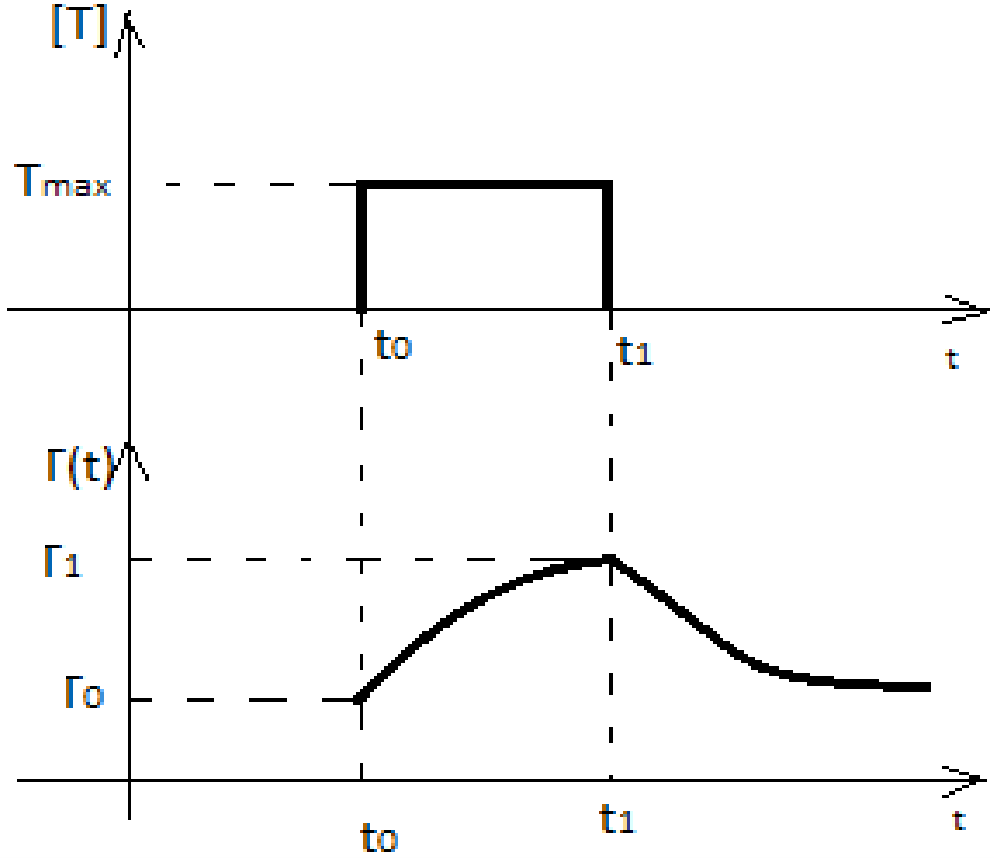
\includegraphics[scale=0.32]{13_2}
    \centering
\end{figure}
A necessary hypothesis is that the release of neurotransmitters is modelled as a pulse,
as depicted in the figure above. The dynamics of \(r(t)\) is given as follow:
\begin{equation*}
    r(t)=
    \begin{cases}
        r_{\infty}+\bigl[r(t_{0})-r_{\infty}\bigr]\cdot{e^{-\frac{t-t_{0}}{\tau_{r}}}}\hspace{1.5cm}\text{for}\;t_{0}\le{t}<t_{1} \\
        r(t_{1})\cdot{e^{-\beta(t-t_{1})}}\hspace{3.5cm}\text{for}\;t\ge{t_{1}}
    \end{cases}
\end{equation*}
where
\begin{equation*}
    r_{\infty}=\frac{\alpha\cdot{[T]_{max}}}{\alpha\cdot{[T]_{max}}+\beta}
    \hspace{3cm}
    \tau_{r}=\frac{1}{\alpha\cdot{[T]_{max}}+\beta}
\end{equation*}
where \([T]_{max}\) is the maximum neurotransmitter concentration in the synaptic cleft.\\
Note that such a model works well without any assumption on the type
of synapses, which might be either excitatory or inhibitory.
\begin{figure}[H]
    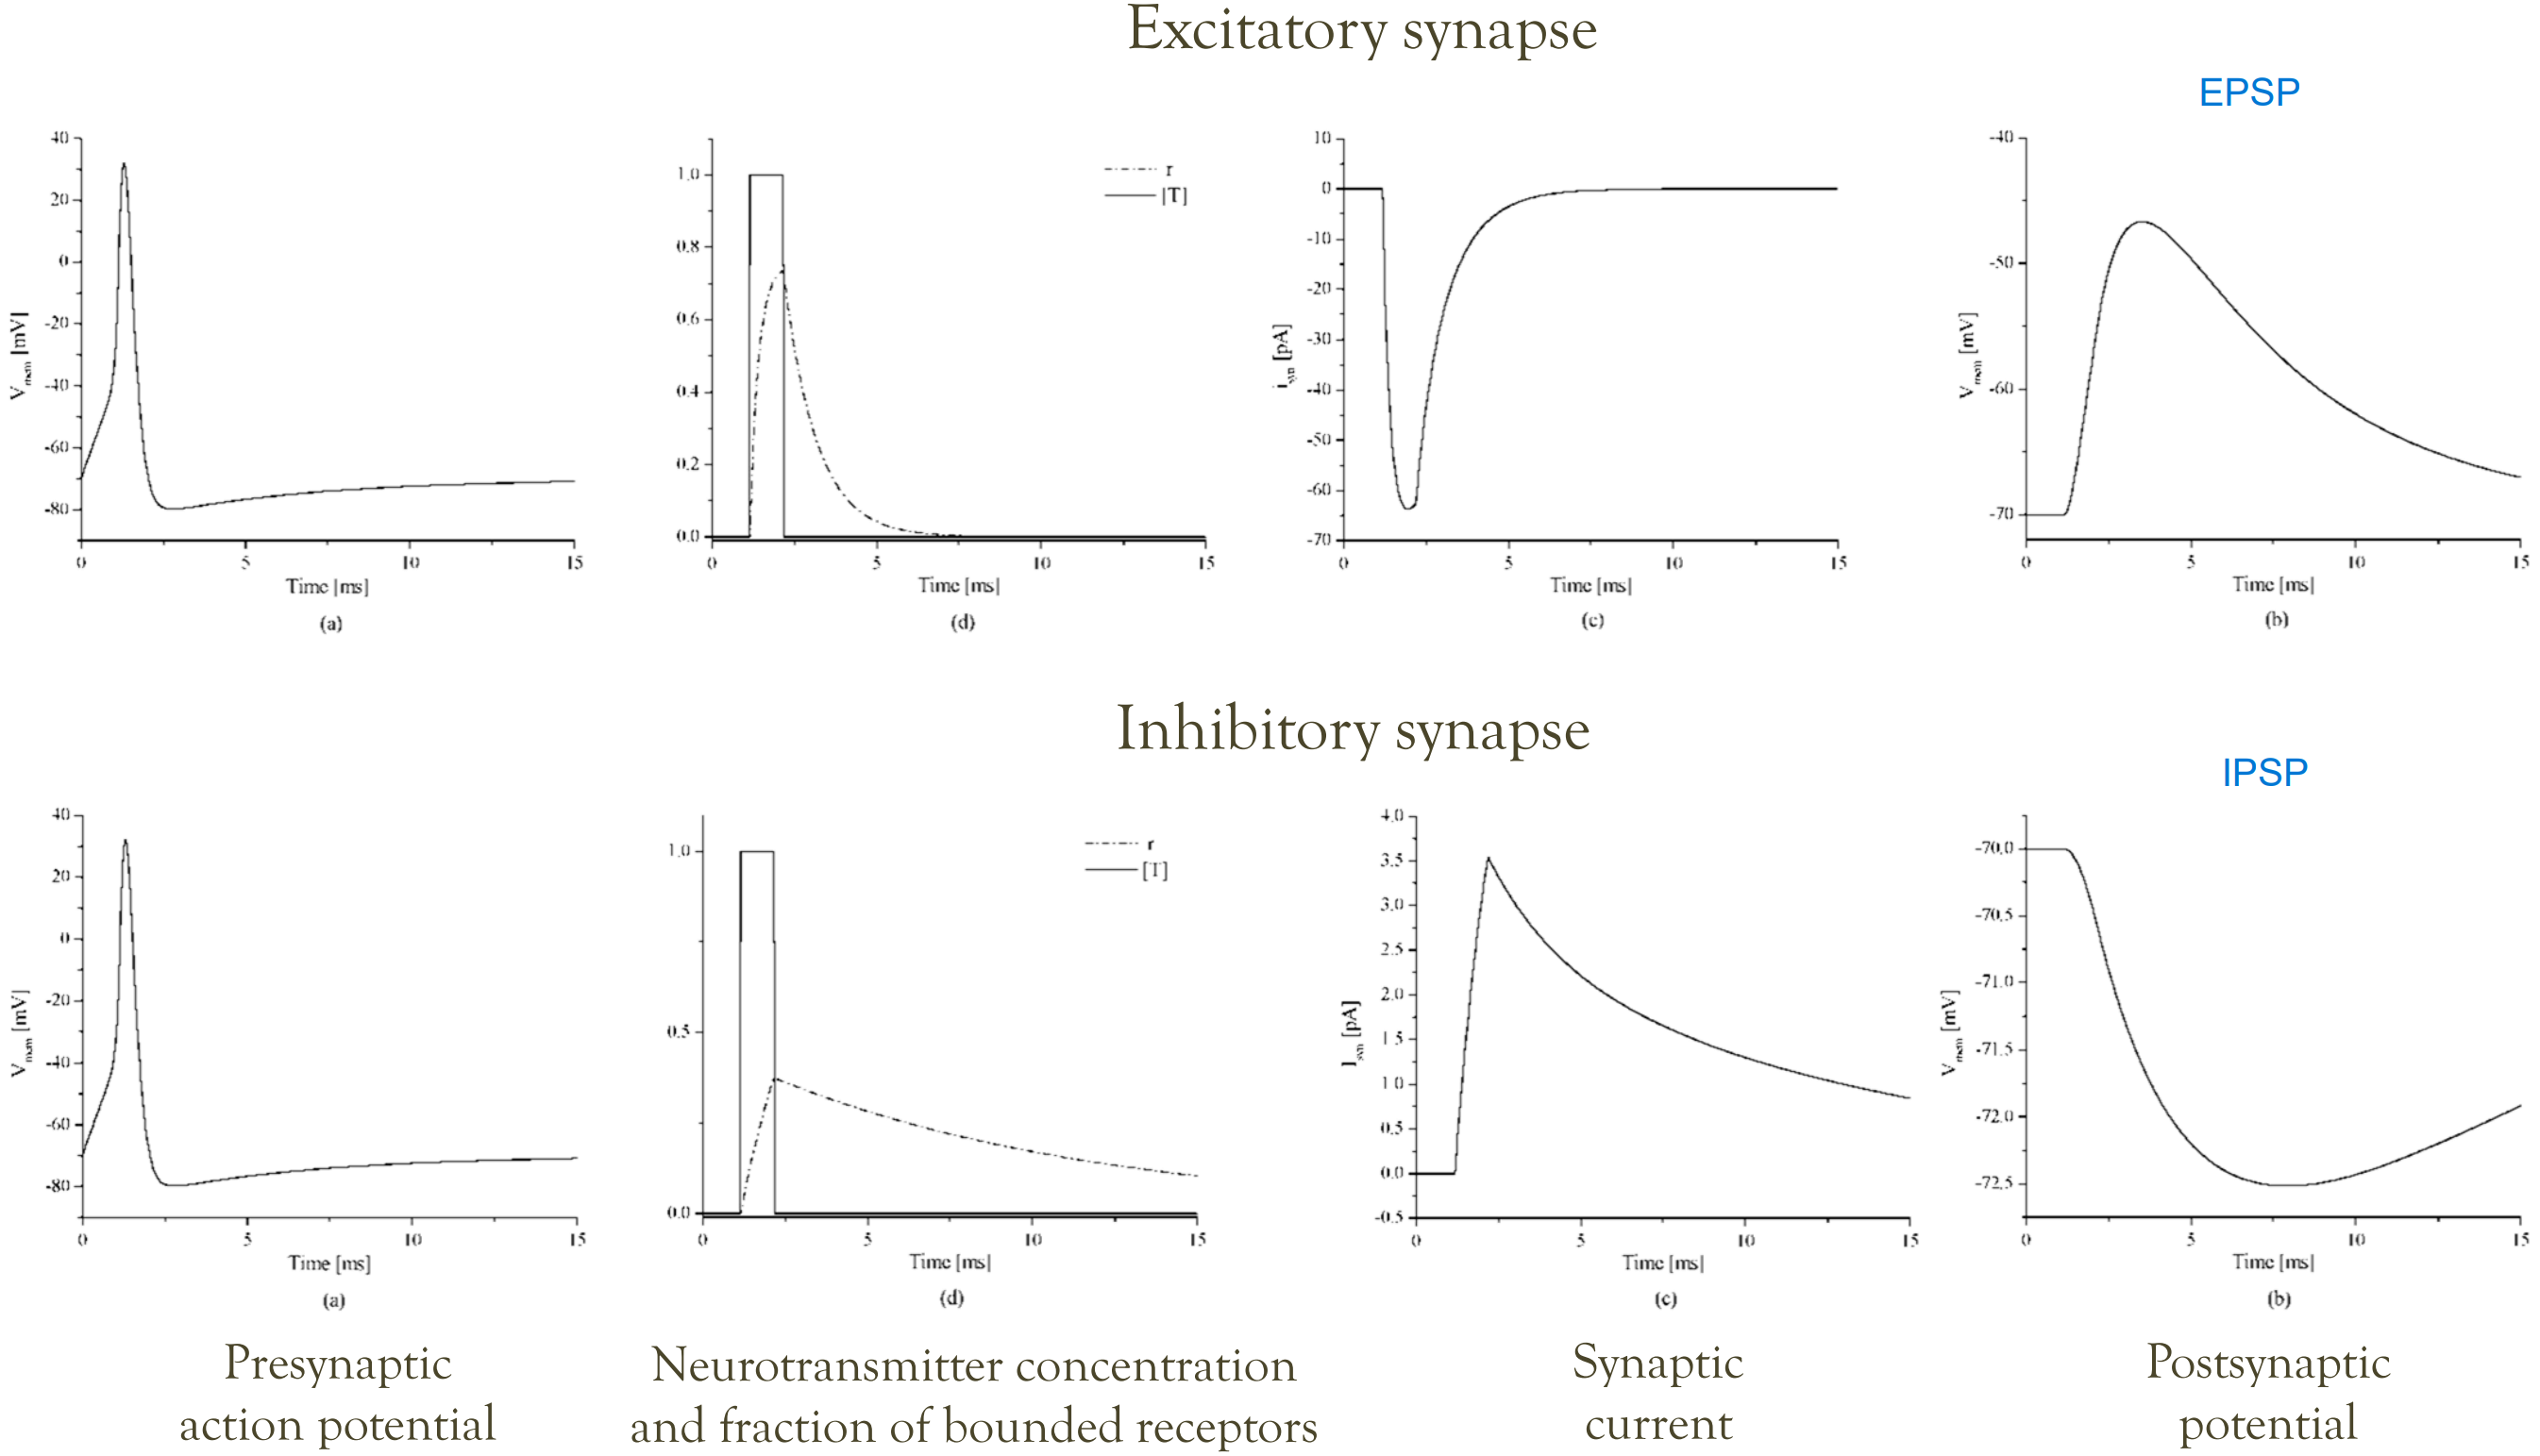
\includegraphics[scale=0.29]{13_3}
    \centering
\end{figure}
In addition to that, this model also allows to easily reprodce the synaptic
integration phenomenon, which is a fundamental property of synapses. If a train
of action potentials is elicited in the presynaptic neuron, this is reflected
as a summation of postsynaptic potentials, eventually causing an action potential
in the postsynaptic neuron whenever the threshold voltage is overcome.
\begin{figure}[H]
    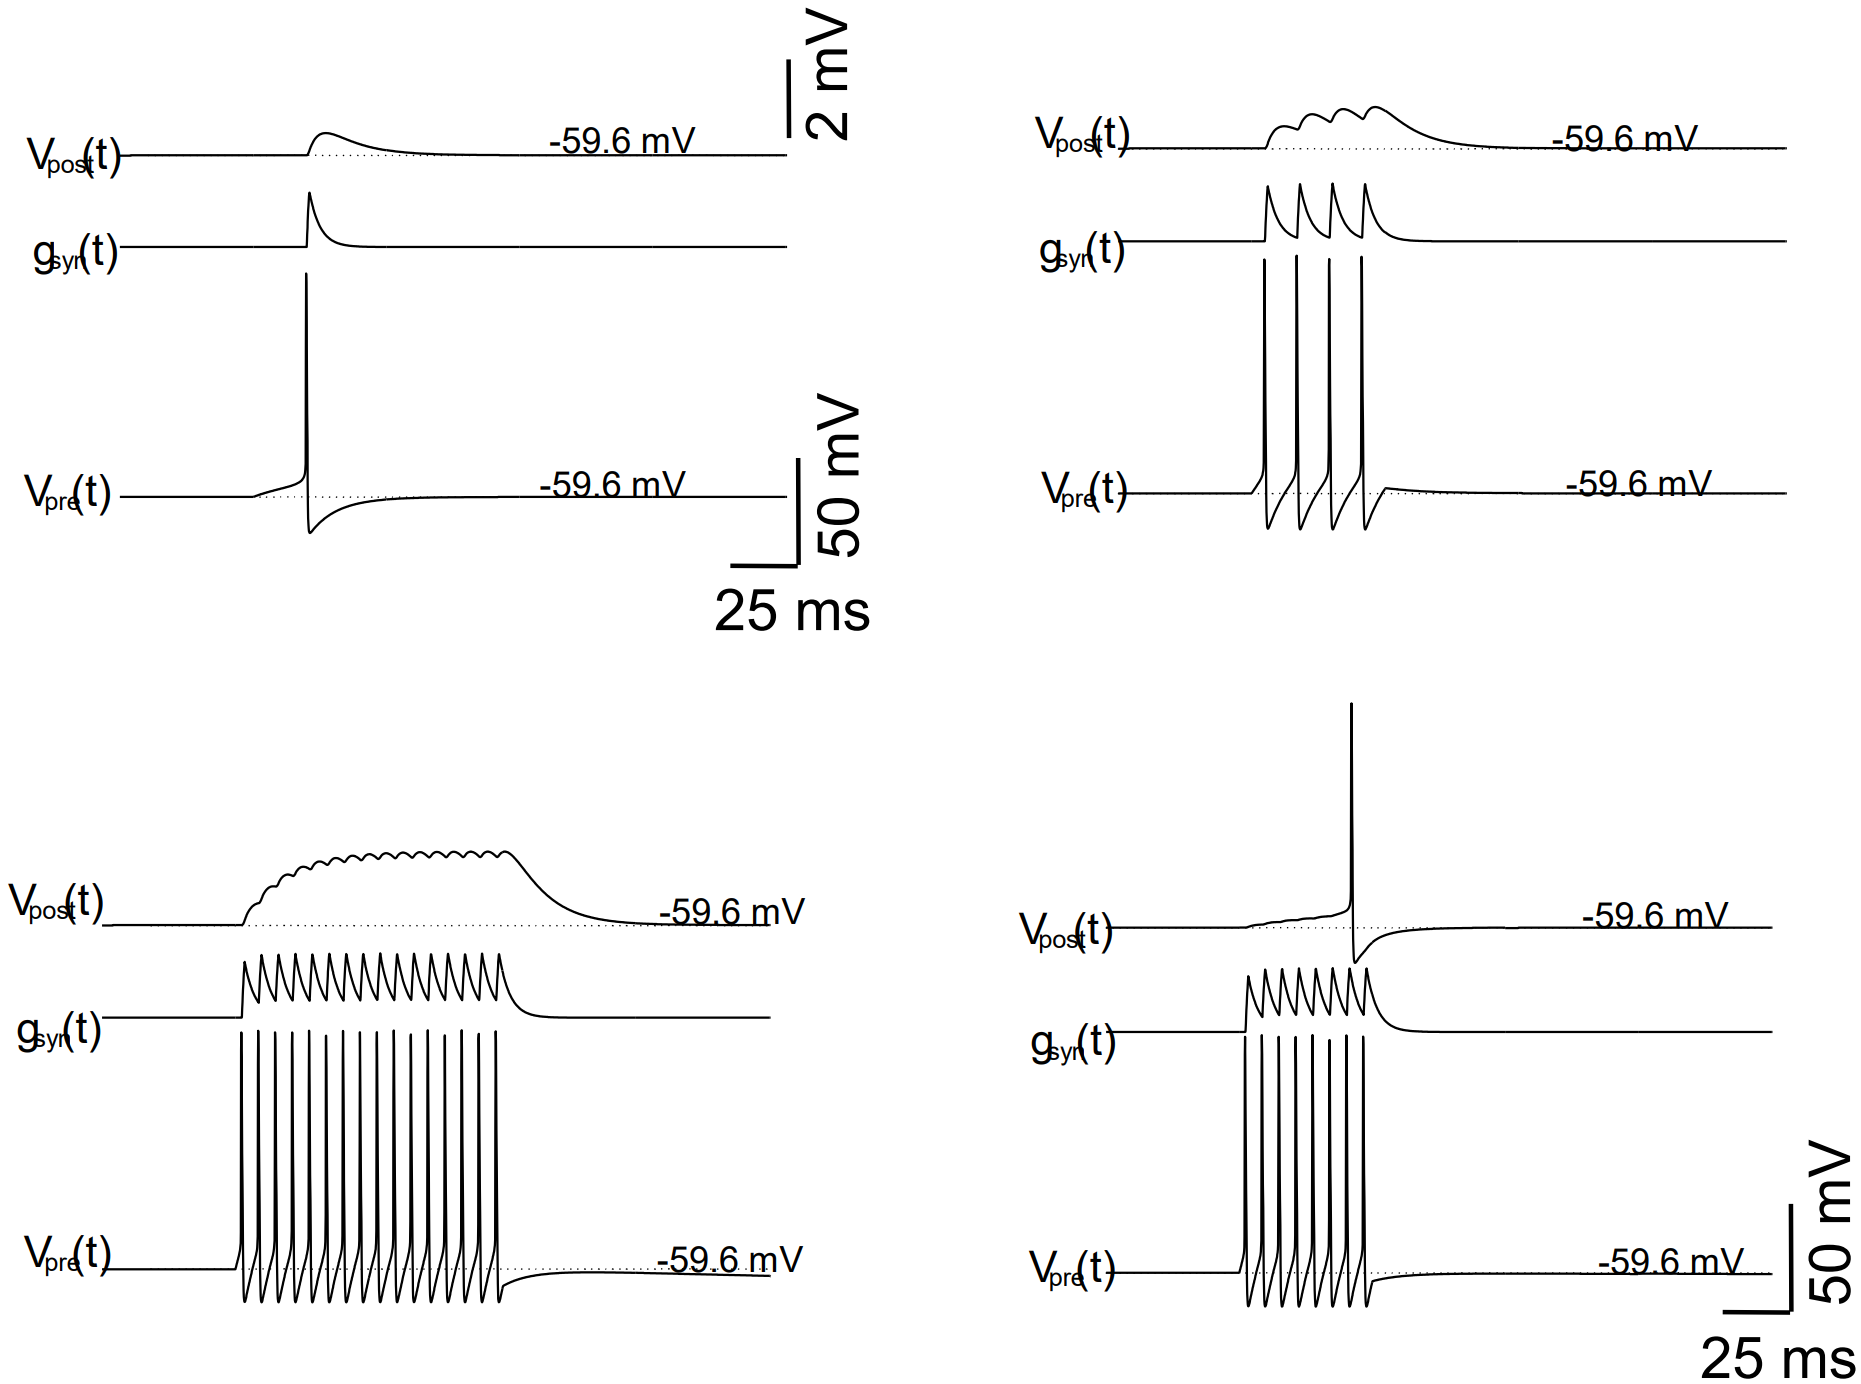
\includegraphics[scale=0.35]{13_4}
    \centering
\end{figure}
The major limitation of the Destexhe model is the fact that the concentration of neurotransmitters is
assumed to be a pulse, however this is not the case from a biological viewpoint. Hence, another
model better modelling what happens at the level of the presynaptic neuron is required.

\subsection{The Yamada-Zucker Model}
This model is focused on modelling the molecular reactions at the presynaptic level, thus
it is curcial to recall the main biochemical steps occurring there:
\begin{enumerate}
    \item Due to an action potential, Ca\({}^{2+}\) ions enter the presynaptic terminal.
    \item These Ca\({}^{2+}\) ions activate calcium-binding proteins (\(X\)) which are able to
          trigger the release of neurotransmitters.
    \item An infinite number of docked vescicles (\(V_{e}\)) are available in the presynaptic terminal,
          ready to release neurotransmitters: this is a \textbf{strong assumption}.
    \item The activated calcium-binding proteins (\(X^{*}\)) bind to the docked synaptic vescicles,
          activating them (\(V_{e}^{*}\)) and causing the release of \(n\) neurotransmitter molecules (\(T\)).
\end{enumerate}
Such a sequence of events can be schematized by the two coupled equations presented in the following:
\begin{gather*}
    4\text{Ca}^{2+}+X\xleftrightarrow{k_{b},\,k_{u}}X^{*}\\
    X^{*}+V_{e}\xleftrightarrow{k_{1},\,k_{2}}V_{e}^{*}\xrightarrow{k_{3}}T
\end{gather*}
where \(k_{i}\) are the so-called rate constants.\\
The overall process is also depicted below.
\begin{figure}[H]
    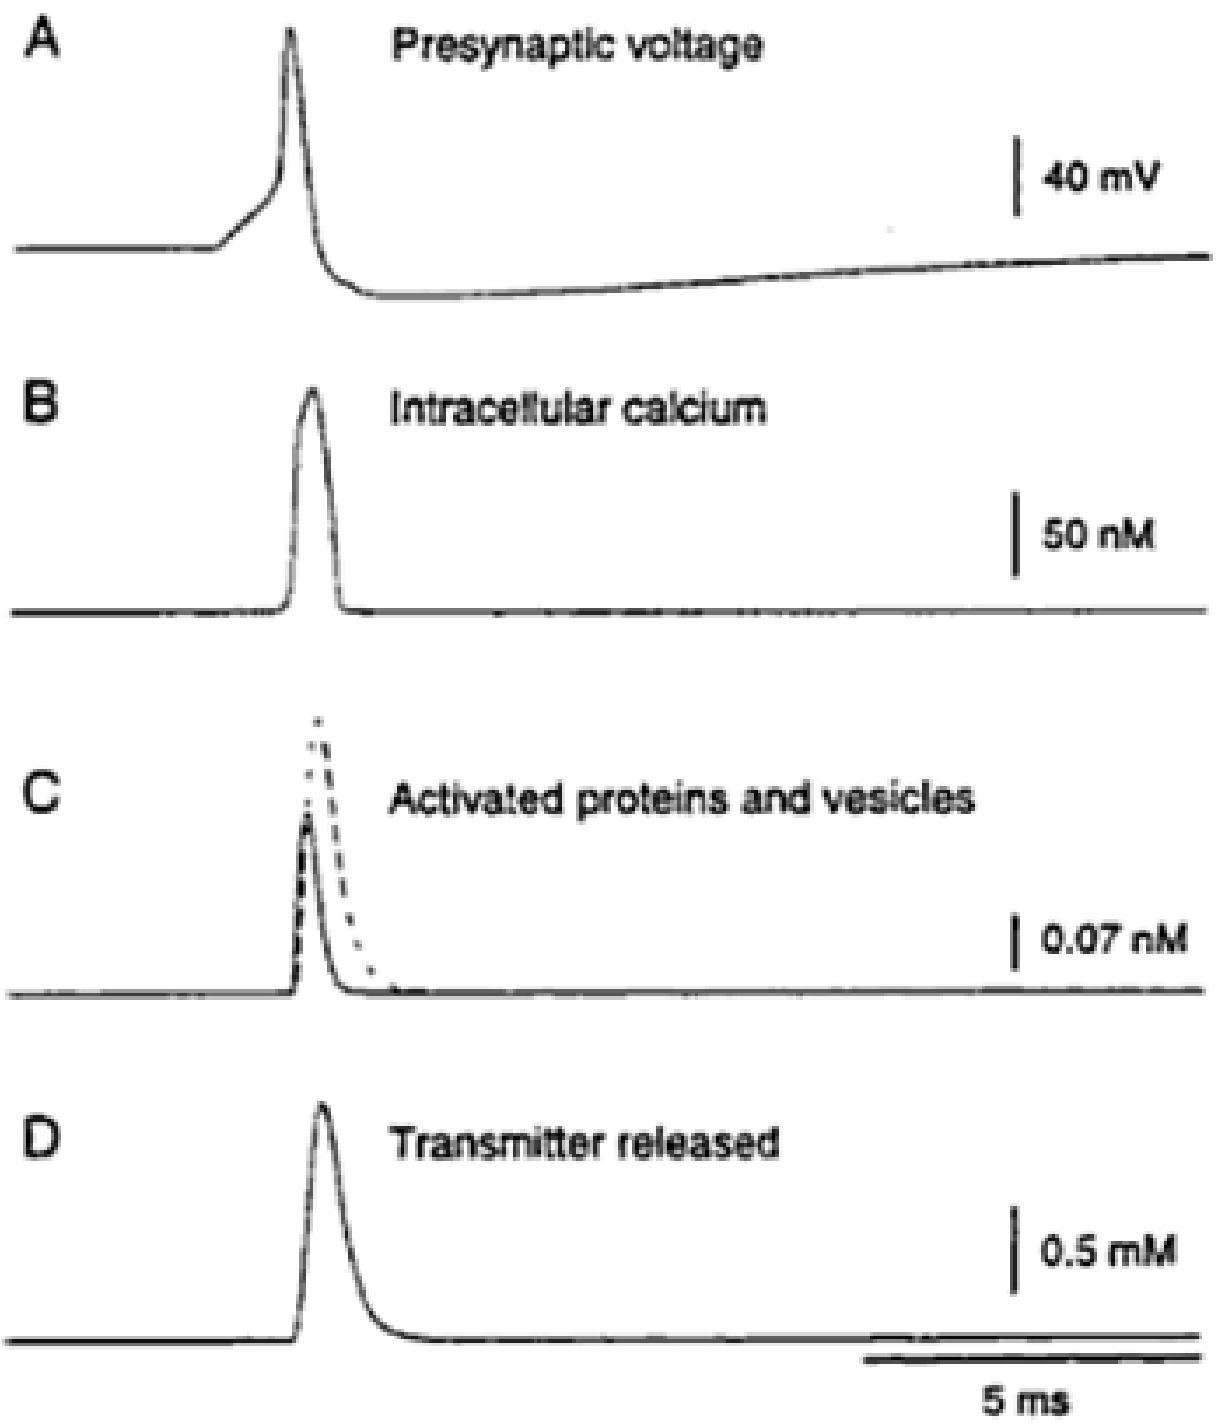
\includegraphics[scale=0.275]{13_5}
    \centering
\end{figure}
Three major assumptions are to be highlighted:
\begin{itemize}
    \item The amount of synaptic vescicles ready to release neurotransmitter molecules
          is infinite.
    \item The concentration of neurotransmitters \([T]\) is assumed to be uniform
          in the synaptic cleft.
    \item The concentration of neurotransmitters \([T]\) in the cleft is cleared
          by processes of diffusion, uptake, degradation, and so on.
\end{itemize}
Finally, the Yamada-Zucker model can be used to describe the concentration of neurotransmitter
molecules to be used as an input parameter for the previously seen Destexhe model: the idea is
to introduce a continuous function to transform the presynaptic neuron membrane potential \(V_{pre}\)
into a neurotransmitter concentration \([T]\). Hence, the neurotransmitter concentration
as a function of the presynaptic voltage can be written as:
\begin{equation*}
    [T](V_{pre})=\frac{[T]_{max}}{1+e^{-\frac{V_{pre}-V_{p}}{K_{p}}}}
\end{equation*}
where \([T]_{max}\) is the maximum neurotransmitter concentration in the cleft, \(V_{p}\) is
the value at which the function is half-activated and \(K_{p}\) models the steepness.

\subsection{Markov Models of Postsynaptic Currents}
One might inquire how to further increase the biophysical accuracy of a synapse model and that can be
achieved by further increasing the complexity of it. In particular, \textit{glutamate} and \textit{GABA}
are well-known to be the principal excitatory and inhibitory neurotransmitters, while the correspondent
postsynaptic receptors are:
\begin{figure}[H]
    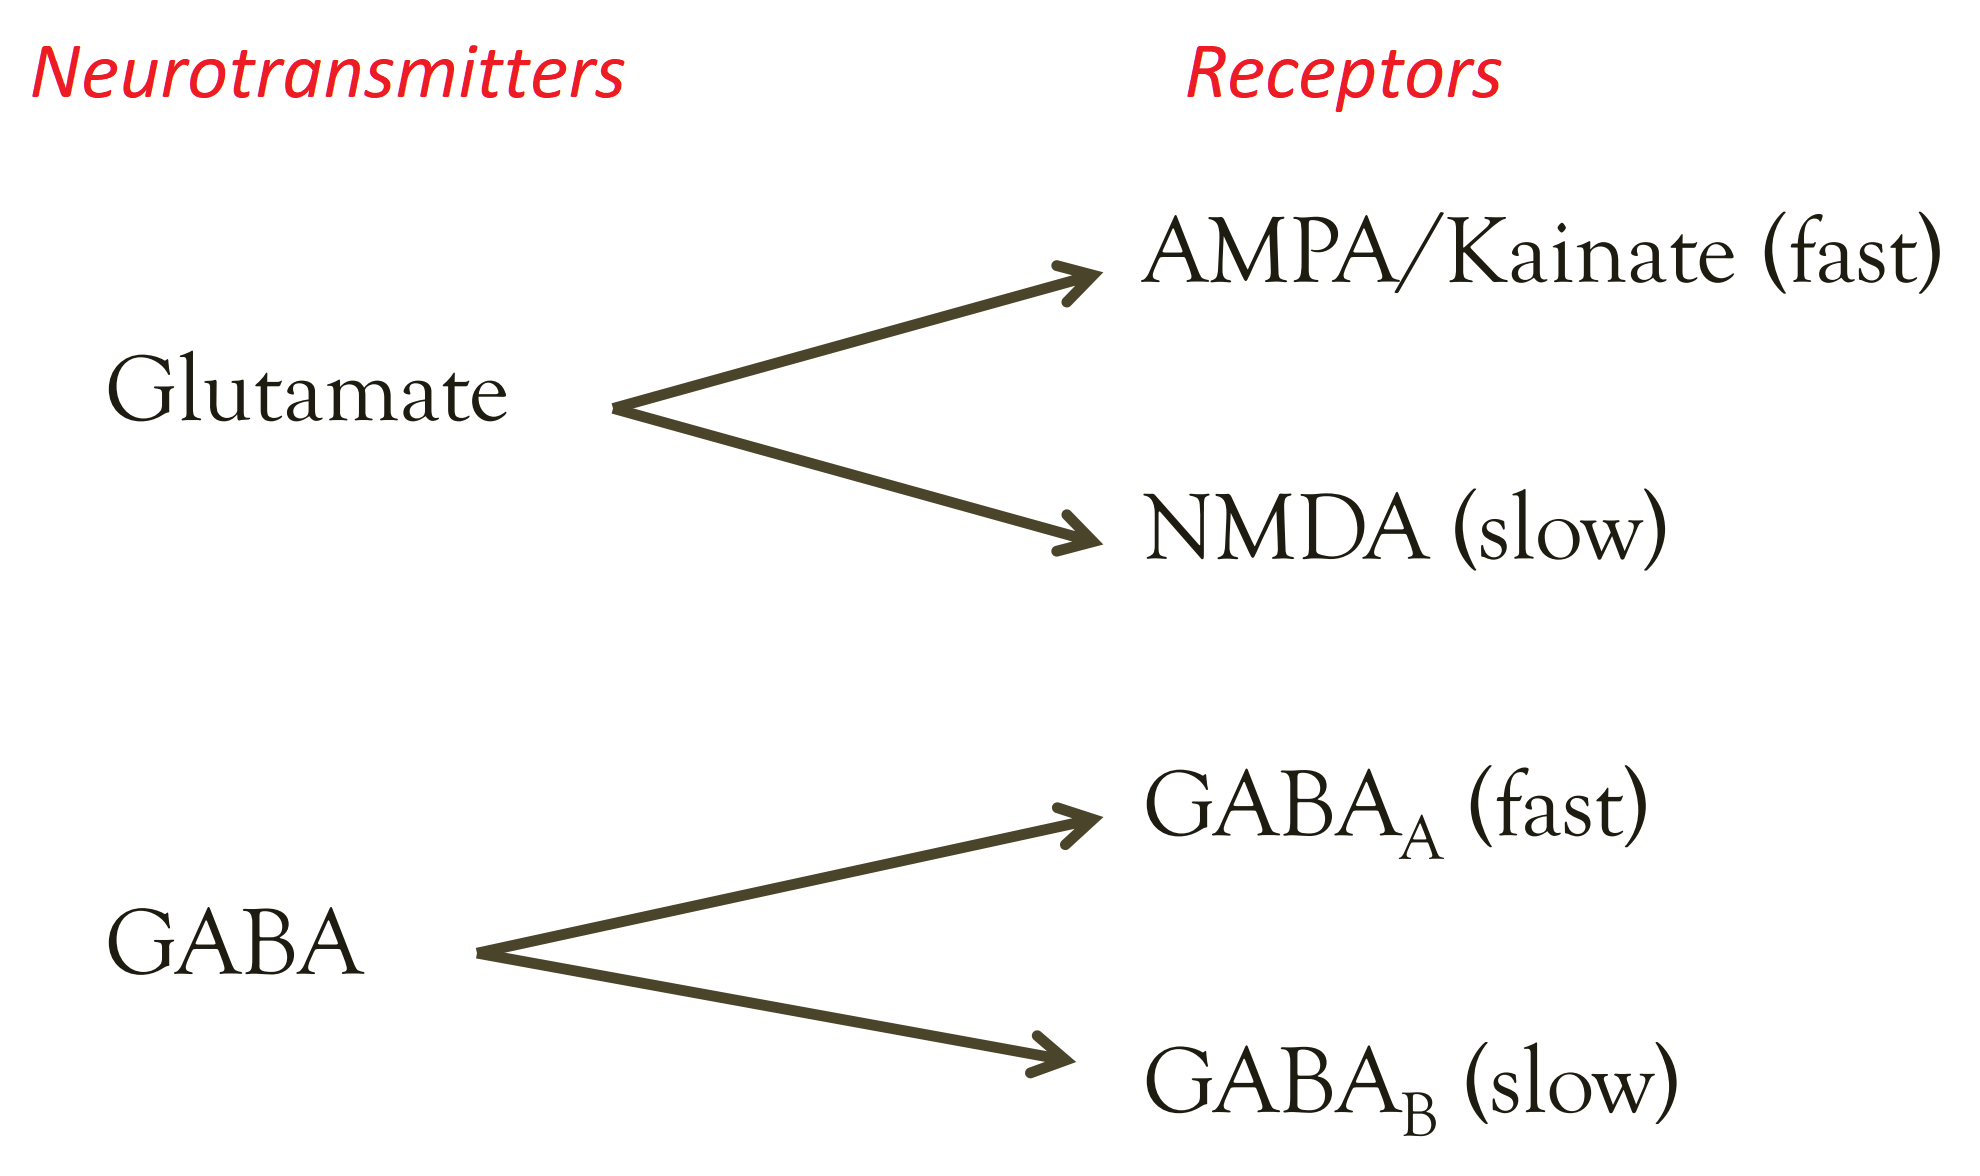
\includegraphics[scale=0.25]{13_6}
    \centering
\end{figure}
Note that each target exhibits different coding features, due to a precise cascade of events.
Unluckily, the Yamada-Zucker model is not able to propely model this cascaded events, therefore
Markov models are introduced. Moreover, a complete model describing the postsynaptic current should
take into account three distinct phases:
\begin{enumerate}
    \item Activation/binding
    \item Deactivation/binding
    \item Desensitization (the synapse is not ready yet)
\end{enumerate}
Marvok models allow to tune the model of a specific receptor to its biological dynamics. Each receptor's
activity goes through different states, according to the type of receptor. Generally, the
postsynaptic current due to a generic receptor \(I_{rec}\) is described by the following formula:
\begin{equation*}
    I_{rec}=\bar{g}_{rec}\cdot{f(...)}\cdot{\bigl(V_{m}-E_{rev}\bigr)}
\end{equation*}
where \(\bar{g}_{rec}\) is the maximum conductance for the considered receptor,
\(E_{rev}\) is the receptor's reversing potential and \(f(...)\) is a function
accounting for the receptor's state, different from type to type.\\
The postsynaptic currents associated with the four kinds of receptors
presented before are the following:
\begin{align*}
    I_{AMPA}     & =\bar{g}_{AMPA}\cdot{[O]}\cdot{\bigl(V_{m}-E_{AMPA}\bigr)}                                   \\
    I_{NMDA}     & =\bar{g}_{NMDA}\cdot{B(V_{m})[O]}\cdot{\bigl(V_{m}-E_{NMDA}\bigr)}                           \\
    I_{GABA_{A}} & =\bar{g}_{GABA_{A}}\cdot{\bigl([O_{1}]+[O_{2}]\bigr)}\cdot{\bigl(V_{m}-E_{\text{Cl}}\bigr)}  \\
    I_{GABA_{B}} & =\bar{g}_{GABA_{B}}\cdot{\frac{[G]^{n}}{[G]^{n}+K_{d}}}\cdot{\bigl(V_{m}-E_{\text{K}}\bigr)}
\end{align*}

\subsection{Modelling the Synaptic Noise}
Spike trains are sometimes modelled according to certain statistic distributions,
commonly the Poisson one. Similar strategies can be adopted to model the
synaptic noise, which was defined in a previous chapter. As a matter or fact, synapses
continuously release a certain amount of neurotransmitters, inducing a response
in the postsynaptic neuron.\\
Noise fluctuations can be added to the model in several ways, but in general a
noisy current representing the synaptic noise is injected in the
postsynaptic neuron. Note that white noise is believed to be the best
candidate in modelling the synaptic noise. Let's define \(\xi_{t}\) as
a white noise with zero mean and unitary variance. Therefore, the noisy
current \(I_{noise}\) is a Gaussian at any time \(t\) and, after a
transient of magnitude \(\tau_{I}\), converges to a process with mean \(m_{I}\)
and standard deviation \(s_{I}\), denominated Uhlenbeck-Ornstein process.
The variation of the noisy current is expressed as:
\begin{equation*}
    dI_{noise}=-\frac{I_{noise}}{\tau_{I}}dt+\frac{m_{I}}{\tau_{I}}dt+s_{I}\sqrt{\frac{2dt}{\tau_{I}}}\xi_{t}
\end{equation*}

\subsection{Biophysical Model for the Tripartite Synapse}
The tripartite synapse refers to the functional integration and physical proximity of
three elements: the presynaptic membrane, the postsynaptic membrane and their intimate
association with surrounding astrocytes. It has been demonstrated that astrocytes
enwrapping synapses can enhance the activity at the synaptic level.
\begin{figure}[H]
    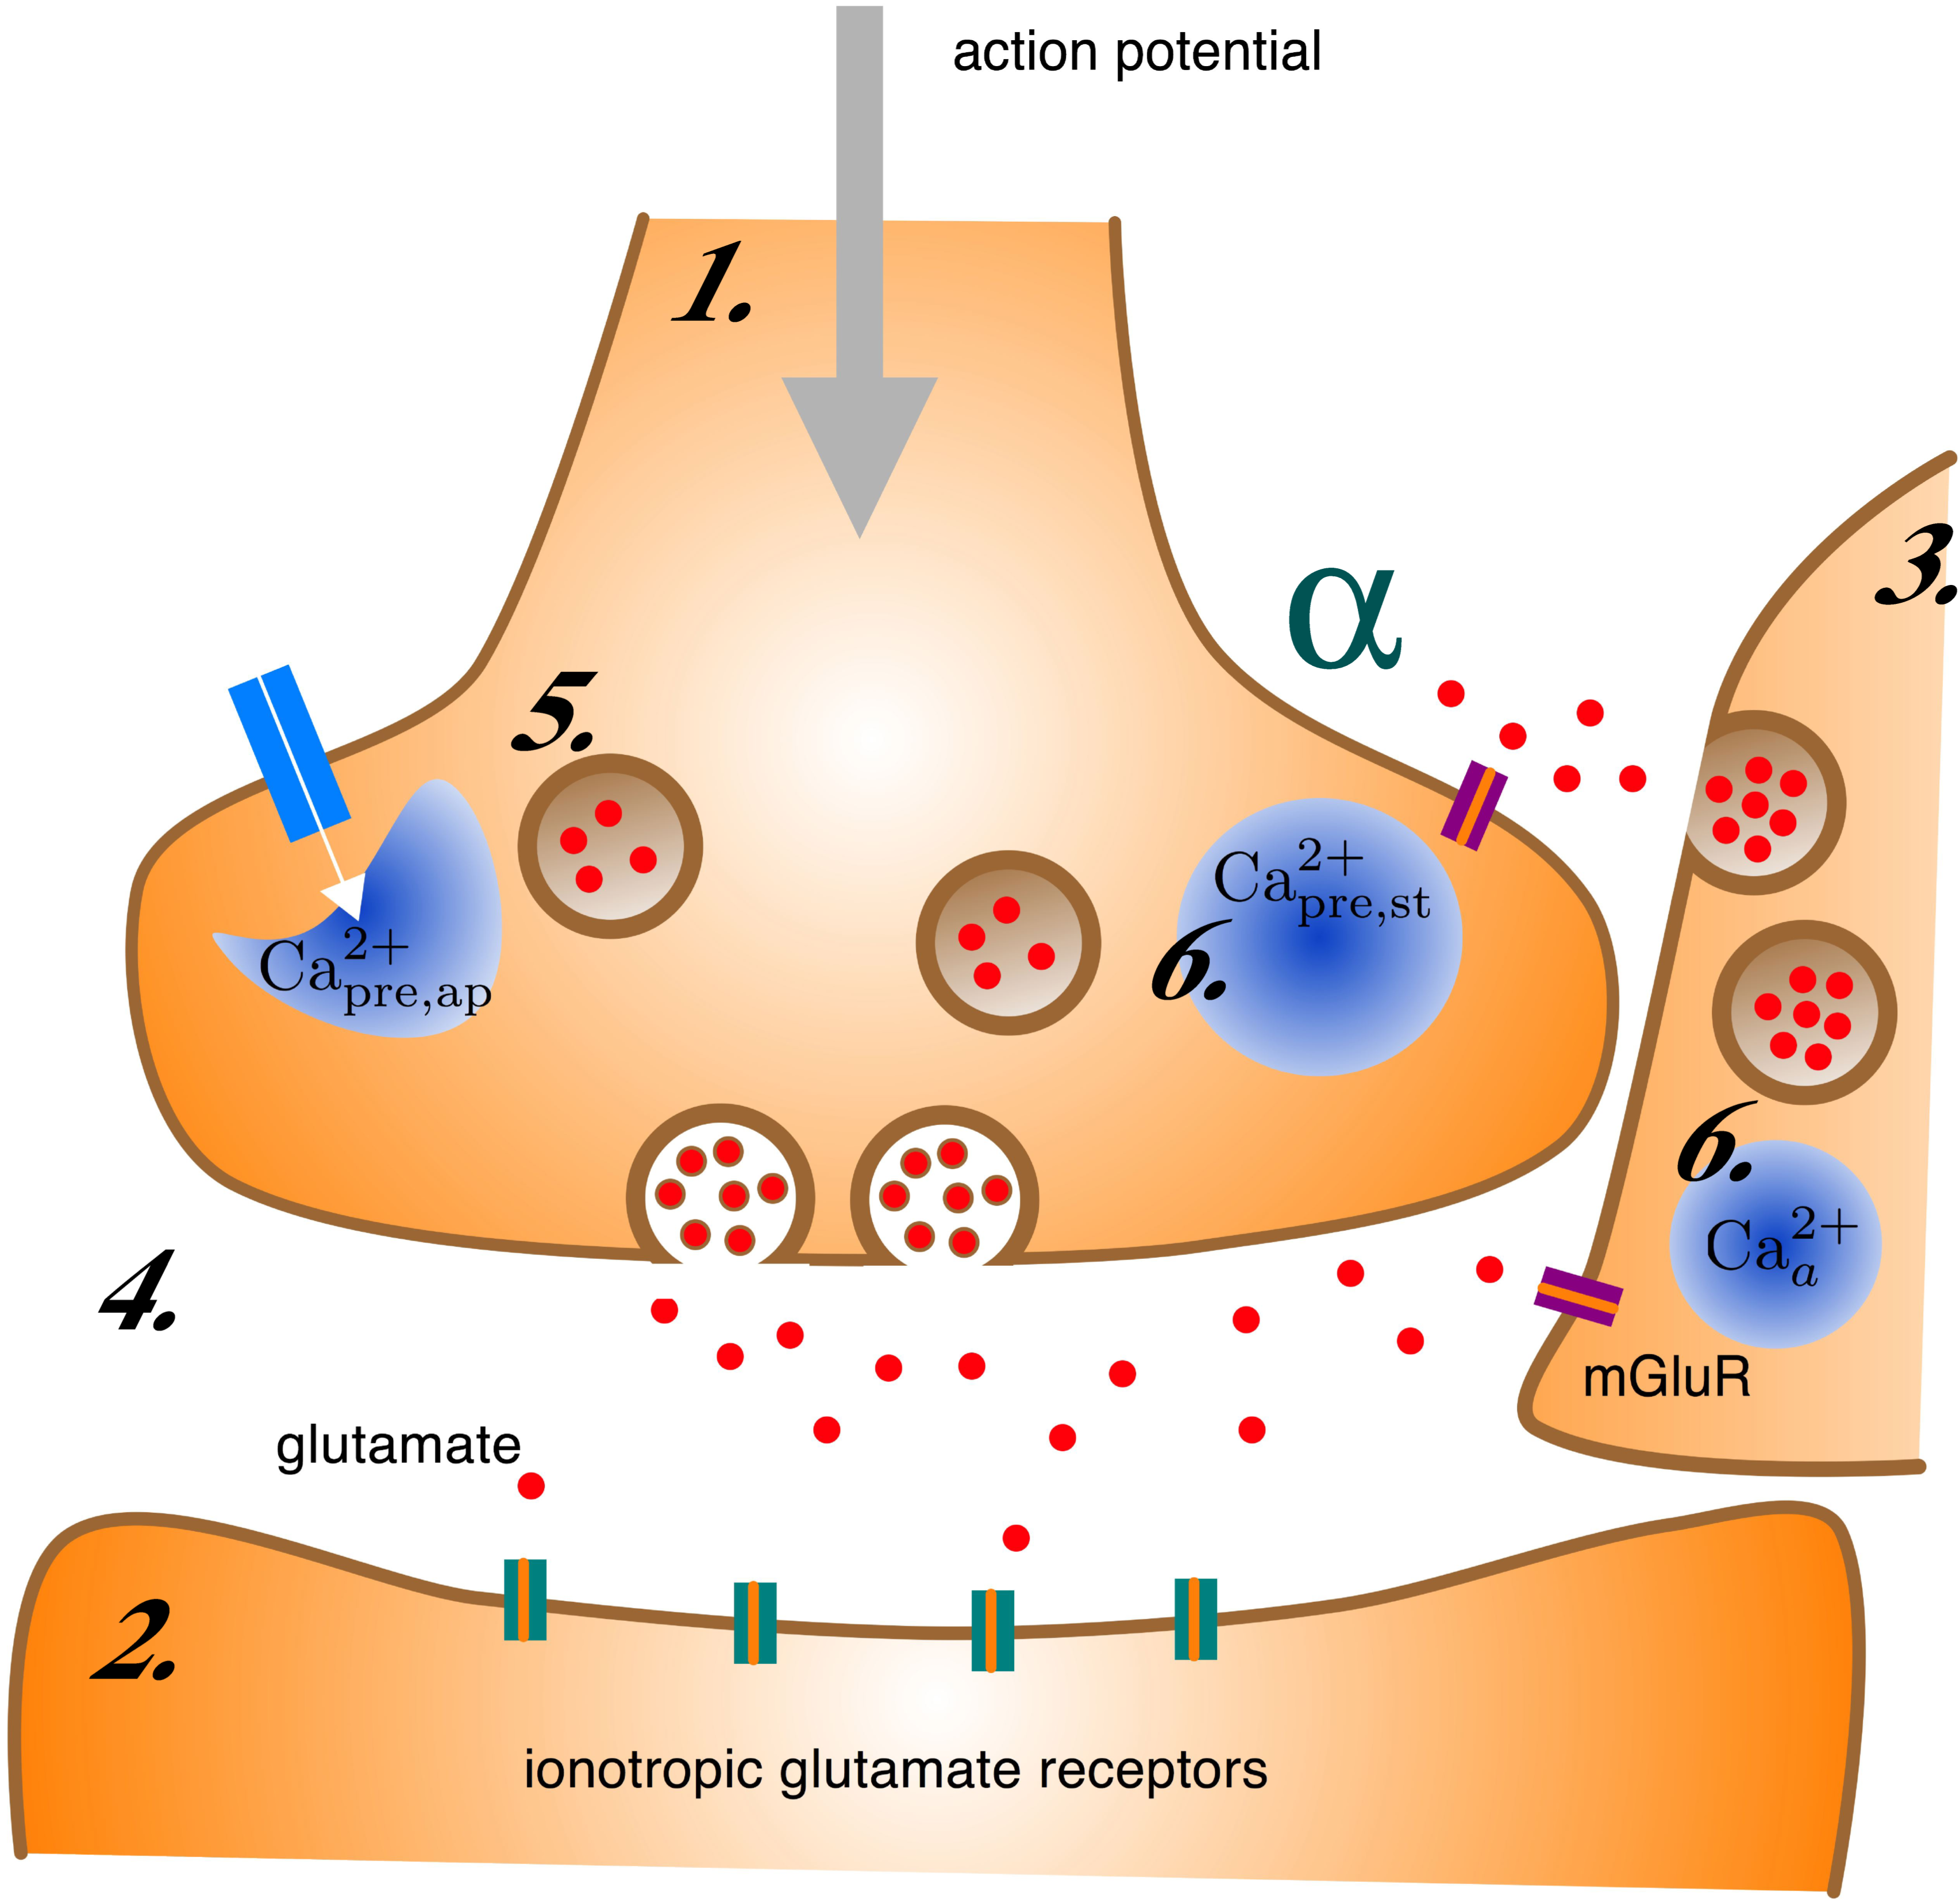
\includegraphics[scale=3.5]{13_7}
    \centering
\end{figure}
The goal is to maximize the induced release in order to maximize the transmission of
information at a synapse and this is accompanied by an increase in the asynchronous
release. Note that both AP-induced and noisy releases draw from the same neurotransmitter
resource pool, thus a large release rate can suppress synaptic transmission via either
depletion of neurotransmitter resources or desensitization of postsynaptic receptors.
Surrounding astrocytes can modulate the probabilities of vescicles release through
bidirectional signaling and hence regulate synaptic transmission.\\
In the following the sequence of steps leading to the potentiation
of the synaptic transmission thanks to an astrocyte is reported:
\begin{enumerate}
    \item Ca\({}^{2+}\) elecation in the astrocyte leads to vescicle-based release of
          glutamate.
    \item Ca\({}^{2+}\) concentration in the presynaptic terminal increases
          due to the activation of presynaptic metabotropic receptors reacting to
          the astrocytically released glutamate.
    \item The vescicle release probabilities are enhanced as a direct consequence
          of the increased presynaptic Ca\({}^{2+}\) concentration.
\end{enumerate}
\subsubsection{The Nadkarni-Jung Tripartite Synaptic Model}
This model aims at describing the behaviour of tripartite synapses.
\begin{itemize}
    \item \textbf{Presynaptic Neuron}: it mimics a hippocampal pyramidal neuron and it is
    described by the two-compartments Pinsky-Rinzel model.
    \item \textbf{Posynaptic Neuron}: it mimics a interneuron and it is modelled by the
    Wang-Buszaki model.
    \item \textbf{Surrounding Astrocyte}: it is not modelled directly, but its enhancing
    behaviour is taken into account by the Nadkarni-Jung model.
\end{itemize}
The presynaptic neuron will release \(N\in\bigl\{0,\,1,\,2\bigr\}\) vescicles
containing glutamate into the synaptic cleft, depending on the presynaptic calcium
ions concentration and on the membrane potential. Each time \(t_{rel}\) a vescicle is
released, glutamate diffuses through the synaptic cleft and binds to postsynaptic
neuron AMPA receptors, eliciting an AMPA current:
\begin{equation*}
    I_{AMPA}=\bar{g}_{AMPA}\cdot{\gamma_{AMPA}}\cdot{\bigl(V_{m}-E_{syn}\bigr)}
\end{equation*}
where \(\gamma_{AMPA}\) describes the first order kinetics of AMPA receptors:
\begin{equation*}
    \frac{d\gamma_{AMPA}}{dt}=\Theta(t-t_{rel})-\Theta(t-t_{rel}-1\,ms)-\frac{\gamma_{AMPA}}{1}
\end{equation*}
Finally, \(I_{AMPA}\) is considered in the postsynaptic neuronal model together with
the other ionic currents and the leakage current.\\
The astrocyte acts whenever the glutamate in the synaptic cleft binds to its
receptors, triggering the release of extra Ca\({}^{2+}\) ions from internal stores
in the cytosol via a second messenger denominated IP\({}_3\). Hence, an
additional source of Ca\({}^{2+}\) ions is introduced and the calcium ions bind to
the postsynaptic receptors.\\
In the following, the results of the tripartite synapse model are reported. In
particular, the presynaptic firing rate was set at \(4\;Hz\) and the AMPA receptor
mediated response is obtained for both the control case - i.e., without astrocytes -
and in the presence of surrounding astrocytes.
\begin{figure}[H]
    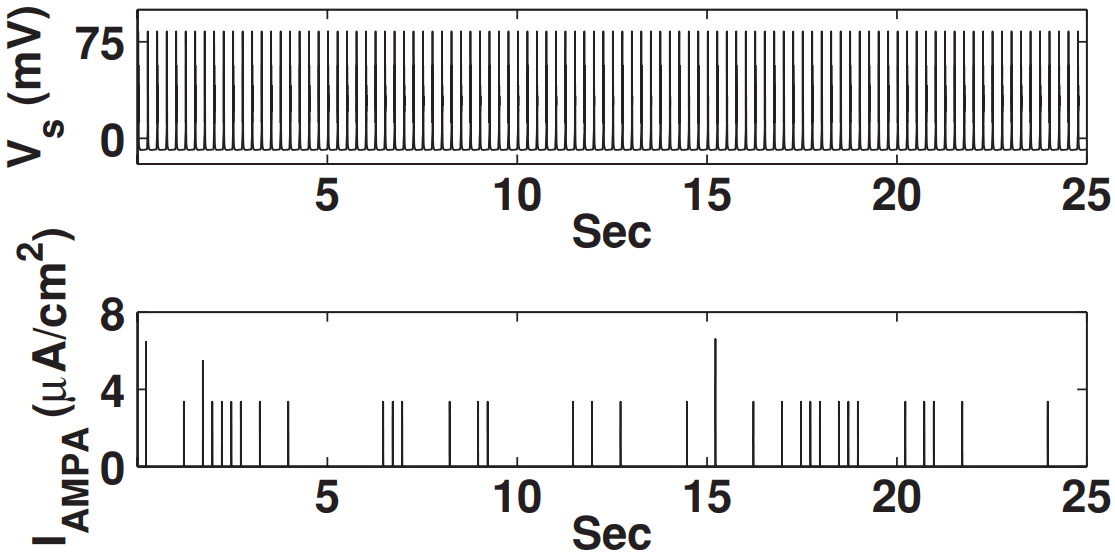
\includegraphics[scale=0.45]{13_8}
    \centering
\end{figure}
The postsynaptic currents do not code very well for the \(4\;Hz\) input spike train,
since only a third of them are transmitted to the postsynaptic terminal.
\begin{figure}[H]
    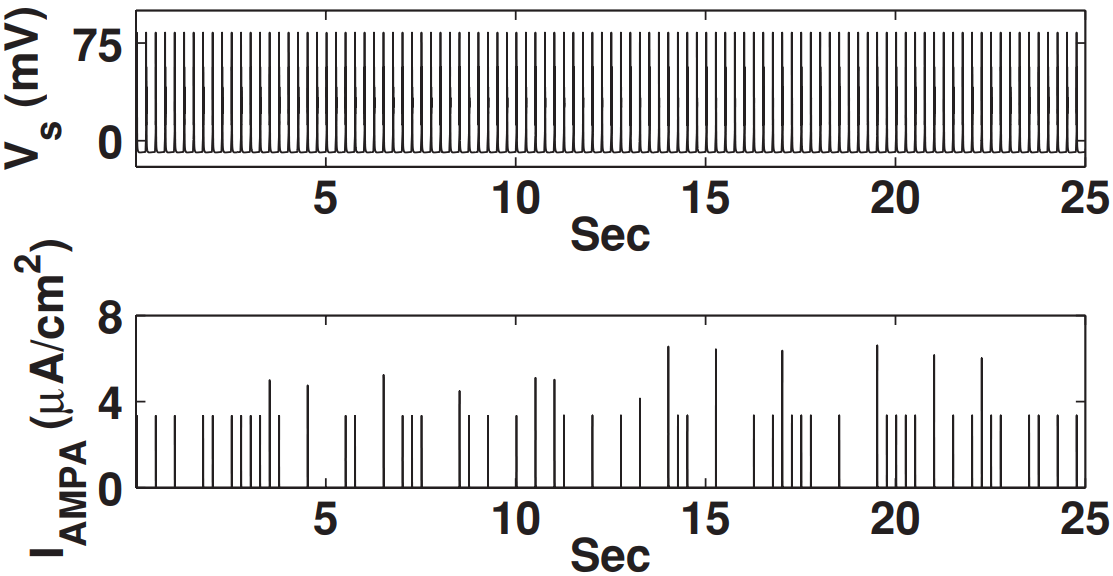
\includegraphics[scale=0.45]{13_9}
    \centering
\end{figure}
In the presence of astrocytes the postsynaptic currents enhance the \(4\;Hz\) input
spike train transmission, hence astrocytes facilitate signal propagation.